\begin{figure}
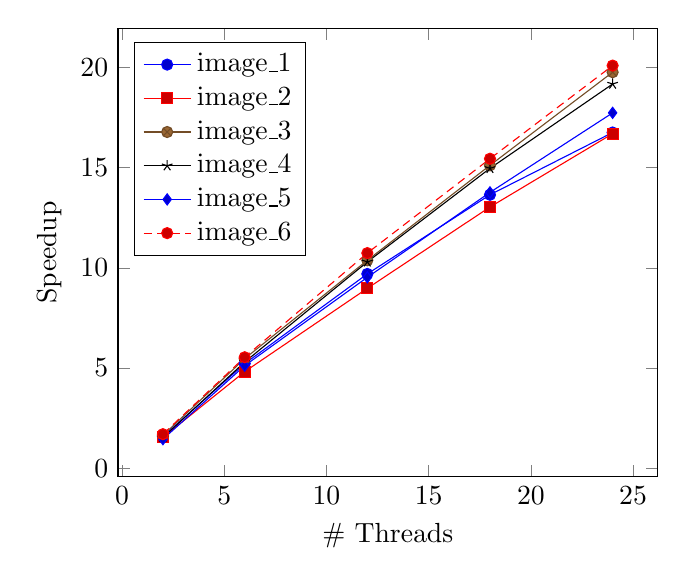
\begin{tikzpicture}
\begin{axis}[legend pos = north west,
xlabel=\# Threads,
ylabel=Speedup]
\addplot+[sharp plot] coordinates {
(2,1.58)
(6,5.22)
(12,9.7)
(18,13.65)
(24,16.76)
};
\addplot+[sharp plot] coordinates{
(2,1.54)
(6,4.82)
(12,8.98)
(18,13.04)
(24,16.70)
};
\addplot+[sharp plot] coordinates{
(2,1.64)
(6,5.47)
(12,10.38)
(18,15.12)
(24,19.77)
};
\addplot+[sharp plot] coordinates{
(2,1.53)
(6,5.30)
(12,10.30)
(18,14.97)
(24,19.18)
};
\addplot+[sharp plot] coordinates{
(2,1.45)
(6,5.12)
(12,9.53)
(18,13.77)
(24,17.74)
};
\addplot+[sharp plot] coordinates{
(2,1.7)
(6,5.54)
(12,10.74)
(18,15.45)
(24,20.10)
};
\legend{image\_1,image\_2,image\_3,image\_4,image\_5,image\_6}
\end{axis}
\end{tikzpicture}
\caption{Speedup for different images and different numbers of threads for local operation}
\label{line}
\end{figure}
